\documentclass{standalone}
\usepackage[single=true, macros=true, xspace=true]{acro}
\usepackage{paralist}
\usepackage{tikz}
\usetikzlibrary{chains, shapes, positioning}

%% Acronym definition example using glossaries package
%% \usepackage{acro} is required
%%
%% For a powerful usage of the acro package look at http://tex.stackexchange.com/questions/135975/how-to-define-an-acronym-by-using-other-acronym-and-print-the-abbreviations-toge
%
% \DeclareAcronym{a}{
%   short = ABC,
%   short-plural = AsBC,
%   long = Acronym Beautifuly Crafted,
%   long-plural = Acronyms Beautifuly Crafteds,
%   cite = {acro_man_url}
% }
%

\DeclareAcronym{mri}{
  short = MRI,
  long  = Magnetic Resonance Imaging
}

\DeclareAcronym{cemri}{
  short = CE-MRI,
  long  = Contrast-Enhanced \ac{mri}
}

\DeclareAcronym{dwi}{
  short = DWI,
  long  = Diffusion-Weighted Imaging
}

\DeclareAcronym{us}{
  short = US,
  long  = Ultra-Sound
}

\DeclareAcronym{nmle}{
  short = NMLE,
  long  = Non-mass-like enhancing
}

\DeclareAcronym{bsp}{
  short = BSP,
  long = Breast Screening Policy,
  long-plural = Breast Screening Policies
}

\DeclareAcronym{cad}{
  short = CAD,
  long  = Computer Aided Diagnosis
}

\DeclareAcronym{dm}{
  short = DM,
  long  = Digital Mammography
}

\DeclareAcronym{gt}{
  short = GT,
  long  = Ground Truth
}

\DeclareAcronym{bus}{
%  short = B\acs*{us},
%  long  = Breast \acifused{us}{\acs*{us}}{\acl*{us}}
short = BUS,
long= Breast Ultra-Sound
}

\DeclareAcronym{ml}{
  short = ML,
  long  = Machine Learning
}

\DeclareAcronym{svm}{
  short = SVM,
  long  = Support Vector Machines
}

\DeclareAcronym{acm}{
  short = ACM,
  long  = Active Contour Model
}

\DeclareAcronym{crf}{
  short = CRFs,
  long  = Conditional Random Fields
}

\DeclareAcronym{mrf}{
  short = MRFs,
  long  = Markov Random Fields
}

\DeclareAcronym{cv}{
  short = CV,
  long  = Computer Vision
}
\DeclareAcronym{icm}{
  short = ICM,
  long  = Iterated Conditional Modes
}
\DeclareAcronym{sa}{
  short = SA,
  long  = Simulate Anealing
}
\DeclareAcronym{gc}{
  short = GC,
  long  = Graph-Cuts
}

\DeclareAcronym{aov}{
  short = AOV,
  long  = Area Overlap
}

\DeclareAcronym{birads}{
  short = BI-RADS,
  long  = Breast Imaging-Reporting and Data System
}

\DeclareAcronym{mad}{
  short = MAD,
  long  = Median Absolute Deviation
}

\DeclareAcronym{qc}{
  short = QC,
  long  = Quadratic-Chi
}

\DeclareAcronym{sift}{
  short = SIFT,
  long  = Self-Invariant Feature Transform
}

\DeclareAcronym{bof}{
  short = BoF,
  long  = Back-of-Features
}

\DeclareAcronym{acr}{
  short = ACR,
  long  = American College of Radiology
}

\DeclareAcronym{fa}{
  short = FA,
  long  = Fibro-Adenoma
}

\DeclareAcronym{dci}{
  short = DCI,
  long  = Ductal Carcinoma in Situ
}

\DeclareAcronym{dic}{
  short = DIC,
  long  = Ductal Inflating Carcinoma
}

\DeclareAcronym{dcis}{
  short = DCIS,
  long  = Ductal Carcinoma in Situ
}

\DeclareAcronym{ilc}{
  short = ILC,
  long  = Inflating Lobular Carcinoma
}

\DeclareAcronym{fpr}{
  short = FPR,
  long  = False Positive Ratio
}

\DeclareAcronym{fnr}{
  short = FNR,
  long  = False Negative Ratio
}

\DeclareAcronym{fp}{
  short = FP,
  long  = False Positive
}

\DeclareAcronym{rbf}{
  short = RBF,
  long  = Radial Basis Function
}

\DeclareAcronym{vicorob}{
  short = ViCOROB,
  long = Computer Vision and ROBotics
}

\DeclareAcronym{florida}{
  short = FSU,
  long = Florida State University
}

\DeclareAcronym{udiat}{
  short = UDIAT,
  long = Centre Diagn\'{o}stic\,-\,Institud Universitary Parc Taul\'i\,-\,UAB
}

\DeclareAcronym{ivim}{
  short = IVIM,
  long  = Intravoxel Incoherent Motion
}

\DeclareAcronym{ecr}{
  short = ECR,
  long  = European Congress of Radiology
}



\begin{document}

% \begin{itemize}
%   \item a \ac{mri}
%   \item a \ac{nmle}
%   \item a \ac{cad}
% \end{itemize}

% \begin{tikzpicture}[]
%   \node[text width = 2cm]{\mri \nmle \cad};
% \end{tikzpicture}



%% Helping functions
%
% CAD schema
\newcommand{\cadSchema}{
    \begin{tikzpicture}[
        start chain=subgroups going below,
        start chain=groups going right,
        every join/.style=->,
        node distance=2mm and 1cm,
      ]
      \node[rectangle split,
          rectangle split parts=3,
          rectangle split part align={right,right,right},
          on chain=groups,
          join
        ]{
          \nodepart{one}T2W-MRI
          \nodepart{two}DWI-MRI
          \nodepart{three}CE-MRI
        };

        \node[on chain=groups,join,draw]{
            \begin{tikzpicture}[
              cadBlock/.style={
                rounded corners, %inner sep=1pt,
                draw, minimum height=4pt, minimum width=3cm
             } ]
              \node[](x){Image Regularization};
              \node[cadBlock, below=3pt of x](a){Pre-processing};
              \node[cadBlock, below=2pt of a](b){Segmentation};
              \node[cadBlock, below=2pt of b](c){Registration};
            \end{tikzpicture}
        };
        \node[on chain=groups,join,draw,minimum width=4cm]{
            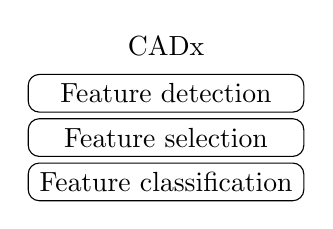
\begin{tikzpicture}[
              cadBlock/.style={
                rounded corners, %inner sep=1pt,
                draw, minimum height=4pt, minimum width=3.5cm
             } ]
              \node[](x){CADx};
              \node[cadBlock, below=3pt of x](a){Feature detection};
              \node[cadBlock, below=2pt of a](b){Feature selection};
              \node[cadBlock, below=2pt of b](c){Feature classification};
            \end{tikzpicture}
        };
    \end{tikzpicture}
}


% Project Flash cards

\newcommand{\impact}
{A novel \cad improving diagnosis of \nmle breast lesions in \mri will reduce medical costs and patient disconfort associated with second look
examinations and biopsies}

\newcommand{\projectScope}
{to develop advanced image analysis techniques for multiparametric \mri to
improve \nmle lesions, disseminate this advances trough open journals and
create value through \ip}

\newcommand{\purpose}
{find physical biomarkers for \nmle breast lesions in multiparametric \mri to
develop novel \cad system}

\newcommand{\team}
{
  \begin{compactitem}[o]
      \item \florida
      \item \vicorob
      \item \udiat
      \item Joan Massich
  \end{compactitem}
}

\newcommand{\success}
{The project would be considered a success if:
  \begin{compactitem}[o]
      \item a multiparametric \mri evaluation framework for \nmle breast lesions is set
      \item potentialy highly citable articles are published
      \item physical biomarkers are found
      \item a comercializable \cad system is created
  \end{compactitem}
}

\newcommand{\resources}
{
  \begin{compactitem}[o]
      \item dataset of 400 patients
      \item oitt
      \item great advisors
      \item clinical validation
      \item creative candidate
      \item i2cvb
  \end{compactitem}
}

\begin{tikzpicture}[
	scale=0.75,
	start chain=1 going below,
	start chain=2 going right,
	node distance=1mm,
	desc/.style={
		scale=0.75,
		on chain=2,
		rectangle,
		rounded corners,
		draw=black,
		very thick,
		text centered,
		text width=8cm,
		minimum height=12mm,
		fill=blue!30
		},
	it/.style={
		fill=blue!10
	},
	level/.style={
		scale=0.75,
		on chain=1,
		minimum height=12mm,
		text width=2cm,
		text centered
	},
	myBlock/.style={
		on chain=1,
    draw,
    rectangle split,
    rectangle split parts=2,
    rectangle split part align={left,center},
    rounded corners,
		very thick,
		minimum height=12mm,
		minimum width=5cm,
		text width=8cm,
    fill=green!10
	},
	wpBlock/.style={
		on chain=2,
    draw,
    rectangle split horizontal,
    rectangle split parts=4,
	},
  xx/.style={rectangle,fill=red}
	every node/.style={font=\sffamily},
]
% \newcommand{\npd}[1]{\nodepart{two} \tikz \node[xx, minimum width=2cm, inner sep=0mm, text width=3cm,draw]{#1};}
\newcommand{\npd}{\nodepart{two}}


\tikzset{aBlockTitle/.style={
    rectangle split, rectangle split horizontal, rectangle split parts=3,
    rectangle split part align={left,left,left},
    rounded corners, fill=gray!50,
    % draw = black,
}}
\tikzset{aBlockAim/.style={
    rectangle split, rectangle split, rectangle split parts=2,
    rectangle split part align={left,left},
    draw = black,
}}

\newcommand{\aimBlock}[7]{
  % \node[on chain=1] {
      \begin{tikzpicture}[start chain=A going right]
  % \begin{scope}[start chain=A going below]

    % \node[aBlockTitle, on chain=A] (title){
    \node[aBlockTitle] (title){
      \nodepart[text width=6cm]{one}#1
        \nodepart[text width=3cm]{two}\tikz{\node[fill=gray!30]{Milestones: #2};}
      \nodepart[text width=3cm]{three}Deliberable: #3
    };

    % \node[aBlockAim, on chain=A]{aim: \nodepart{two} #4};
    \node[text width=11cm, draw, anchor=north] (aim) at (title.south){#4};
    %
    \node[aBlockAim, on chain=A, anchor=north west, text width=3cm] at (title.west|-aim.south){Actions: \nodepart{two} #5};
    \node[aBlockAim, on chain=A, text width=6cm]{Risks and Alternatives: \nodepart{two} #6};
    \node[aBlockAim, on chain=A, text width=3cm]{impact: \nodepart{two} #7};

    \end{tikzpicture}
  % \end{scope}
  % };
}


%% Start the drawing
%
% Project flashcards
\node [myBlock] (purpose) {Purpose \npd{\purpose}};
\node [myBlock] (projectScope) {Scope \npd{\projectScope}};
\node [myBlock] (impact) {Impact \npd{\impact}};
\node [myBlock] (success) {Success criteria \npd{\success}};
\node [myBlock] (team) {Team \npd{\team}};
\node [myBlock] (resources) {Resources \npd{\resources}};

%
% CAD schema
\node[anchor=north west, xshift=2pt] (cad) at (purpose.north east){\cadSchema};


%% Aim and WorkPackages
%
\tikzset{aBlock/.style={ on chain=2, draw, very thick, rounded corners}}

%
% Aim 1: Evaluation Benchmark
\node[aBlock, anchor=north west, yshift=-4pt] (aim1) at (cad.south west){
  \aimBlock{Evaluation Benchmark}
  {mst}
  {zz}
  {Cover the lack of standerized platform for testing breast lesions diagnosis when using multiparametric \mri.}
  {\begin{compactitem}[o]
      \item Publishable dataset
      \item Evaluation metric
      \item MICCAI Challenge
    \end{compactitem}}
  {If the challenge is canceled, a local challenge will be organized at MaIA}
  {\begin{compactitem}[o]
      \item Benchmark for our CAD
      \item Scientific publication likely to be highly cited
    \end{compactitem}}
};
\chainin (aim1);

%
% Aim 2: 
\node[on chain=2,continue chain=going below]{
  \aimBlock{Title}
  {mi.st}
  {delib.}
  {aim of this block}
  {Actions for this block}
  {Riscks and alter.}
  {impact}
};

%
% Aim 3: 
\node[on chain=2,continue chain=going below]{
  \aimBlock{Title}
  {mi.st}
  {delib.}
  {aim of this block}
  {Actions for this block}
  {Riscks and alter.}
  {impact}
};





% \aimBlock{xx}{yy}{zz}{kk}{5}{6}{7}{8}


% \node [draw] (aim1) {
% \aimBlock{xx}{yy}{zz}{kk}
% };

% % Levels
% \node [level] (Level 5) {Level 5};
% \node [level] (Level 4) {Level 4};
% \node [level] (Level 3) {Level 3};
% \node [level] (Level 2) {Level 2};
% \node [level] (Level 1.5) { };
% \node [level] (Level 1) {Level 1};
% \node [level] (Level 0) {Level 0};

% % Descriptions
% \chainin (Level 5); % Start right of Level 5
% % IT levels
% \node [desc, it] (Archives) {Archives/File Servers};
% \node [desc, it, continue chain=going below] (ERP) {ERP/Finance/Messaging};
% % % ICS levels
% % \node [desc] (Operations) {Operations Management/Historians};
% % \node [desc] (Supervisory) {Supervisory Controls};
% % \node [desc, text width=3.5cm, xshift=2.25cm] (PLC) {PLC/RTU IP Communication};
% % \node [desc, text width=3.5cm, xshift=-4.5cm] (SIS) {Safety Instrumented Systems};
% % \node [desc, xshift=2.25cm] (IO) {I/O from Sensors};

\end{tikzpicture}
\end{document}
